\chapter{Preliminary Analysis} \label{chapter:preliminary}
This Chapter presents the data sources, data fetching method, initial description of the raw data, as well as data analysis and visualization methods. For demonstration, we use the dataset includes limit order book data, market trade book data and MN trade book data from 10:00:00 to 15:59:59 on 31st January as examples. The timestamps in the order book and MN trade book are recorded in London time, while those in the market trade book are American time. To ensure orders in order book are consistent with trades in trade book, all of them are converted to Central European Time (CET). As a result, bot them represent for trading time between 10:00:00 and 15:59:59 CET. 

In Section~\ref{sec:data-source}, data structures are shown in tables, alongside brief description and data type. Then in Section~\ref{sec:match-order-trade}, we describe how trades in the trade book are matched with the orders in the order book. We build an algorithm to find this match by comparing trade prices and directions with the prices in different levels of the order book. We also classify visible trades into passive and aggressive types based on whether the match happens at the best bid/ask price. 
In Section~\ref{sec:price}, we explain the trading activity using the price and filling information from order book and trade book data. This helps us visualize how aggressive and passive trades appear and interact with mid-price movements and spread dynamics in the data. 


\section{Data Source and Types} \label{sec:data-source}
The order book dataset consists of foreign exchange (FX) limit order book data provided by LMAX and CBOE, two venues used by MN. Orders from LMAX is more transparent because LMAX is optimized for order-driven market model, while there are more latent orders in CBOE because of the support for anonymous trading. 

As can be seen in Table~\ref{tb: order book data description}, the currency type is EUR/USD. The data is detailed in bid/ask prices and volumes at 5 levels in total, where the data of level 1 stand for the best bid/ask. The dataset also calculates the spread between best ask and best bid prices.

\begin{table}[h]
    \centering
    \begin{tabular}{lll}
        \toprule
        \textbf{Column} & \textbf{Description} & \textbf{Data Type} \\
        \midrule
        ID & Unique identifier of orders & String \\
        $T$ & Time of the snapshot in HH:MM.S format & String \\
        VENUE & The exchange (LMAX or CBOE) & String \\
        SYMBOL & Currency pair (EUR/USD) & Datetime \\
        $V_A$ & Total volume on the ask side & Integer \\
        $V_B$ & Total volume on the bid side & Integer \\
        $P_A ^ {i}$, $i = 1, \dots, 5$ & Ask prices at different levels & Float \\
        $V_A ^ {i}$, $i = 1, \dots, 5$ & Corresponding volumes at each ask level & Integer \\
        $P_B ^ {i}$, $i = 1, \dots, 5$ & Bid prices at different levels & Float \\
        $V_B ^ {i}$, $i = 1, \dots, 5$ & Corresponding volumes at each bid level & Integer \\
        $S$ & Difference between best ask and bid (S = $P_A ^ {1}$ - $P_B ^ {1}$) & Float \\
        \bottomrule
    \end{tabular} 
    \caption{Order Book Data Description}
    \label{tb: order book data description}
\end{table}

All the order book data is stored in Snowflake, a cloud-based data platform that provides data storage, processing, and analytics as a fully managed service. High-frequency order book data can be accessed using SQL queries, which ensures high availability and completeness of data.

Unlike the limit order book data, the trade book data only contains trades executed on the CBOE. In the Table~\ref{tb: trade book data description}, it provides information of trade price, volume, execution time, and order direction. Since CBOE supports anonymous trading, the trade book may contain hidden order executions that are not visible in the limit order book updates.

\begin{table}[h] 
    \centering 
    \begin{tabular}{lll} 
        \toprule 
        \textbf{Column} & \textbf{Description} & \textbf{Data Type} \\ 
        \midrule 
        $T$ & Execution time of the trade (HH:MM:SS) & String \\
        DIRECTION & Bid order or ask order & String \\
        PRICE & Execution price of the trade & Float \\ 
        VOLUME & Number of units traded & Integer \\  
        \bottomrule 
    \end{tabular} 
    \caption{Trade Book Data Description}
    \label{tb: trade book data description}  
\end{table}

\section{Matching Trade Book and Order Book Data} \label{sec:match-order-trade}
In an order-driven market, trades occur when incoming orders match existing orders in the order book. In the \gls{lob}, 'bid' represents buy interest, and 'ask' represents sell interest. When a trade is recorded in the trade book, it has a direction. If the direction is 'Bid', it means the buyer placed an order that matched an existing ask order in the order book. In this case, the trade price corresponds to the ask price available in the order book at the time of execution, and the volume of the matched ask order decreases by the traded amount. If the direction is 'Ask', it means the seller placed an order that matched an existing bid order in the order book. The trade price in this case corresponds to the bid price available in the order book, and the volume of the matched bid order decreases by the traded amount. The order book is updated after each trade to reflect the reduced volume of the matched order. If an order in the order book is fully consumed, it is removed. If there is remaining volume after a partial match, the order stays in the book with the updated volume. 

An algorithm is developed to find roots of trade book updates in the order book data. This is an important preliminary to see how orders in the order book get filled, which is important in back testing. Also, it is clear to see how many unmatching orders in the order book are. The algorithm for matching orders and trades is in Algorithm~\ref{alg:trade_order_matching}.

\begin{algorithm}
    \caption{Matching Trade Book and Order Book Data}
    \label{alg:trade_order_matching}
    \begin{algorithmic}[1]
        \State Load trade book (timestamp, price, volume, direction)
        \State Load order book (timestamp, price levels, volumes)
        \State Filter data for CBOE venue and set time range
        \State Convert timestamps to datetime format
        \State Transform order book to long format (one row per price level)
        \State Merge and sort trade book and order book by timestamp
    
        \For {each trade}
            \State Find earlier matching limit orders
            \If {no matching order exists}
                \State Mark as hidden order
            \Else
                \State Check if buy trade matches ask or sell trade matches bid
                \State Record matched price level and traded volume for updates in trade book
                \State Record filling time and traded volume for updates in order book
            \EndIf
        \EndFor
    
        \State Define visible orders: trades that match existing limit orders
        \State Define hidden orders: trades with no matching limit order
        \State Define aggressive orders: visible trades not at best bid/ask
        \State Define passive orders: visible trades at best bid/ask
    
    \end{algorithmic}
\end{algorithm}

It starts by loading and filtering data, selecting only CBOE data within a defined time range for consistency. To identify matching trades, the algorithm checks whether each trade price appears in the five bid/ask levels of the order book. Since order book data stores prices and volumes separately, it is melted into a long format, aligning price levels with corresponding volumes. Then the trade book and order book are then merged into a complete order-trade dataset to accelerate direct comparison.

For each trade, the codes find previous orders in the order book, and check if price and direction match. The bid in the trade book should match the ask in the order book, the ask in the trade book should match the bid in the order book. As the result, If a trade matches an order, it is a visible execution. But if the matching price level is not the best bid or ask, it's identified as a passive submission getting filled by either market movements or aggressive market order. Further classification about these two scenarios will be done later in the chapter 4. If a trade cannot find its root in the order book, it's hidden orders, but we don't really care about this part.

As can be seen in the pie chart \ref{fig:p_of_AT_unma}, hidden trades only account for 3.5\%. Most trades are visible, which shows the high data quality from CBOE. Passive submission and neutral submission are both visible trades which we can find in the order book. Half of them are rooted as passive submission, which shows half traders are willing to queue in the order book flow and either wait for market movements or being chosen by aggressive traders. Half of the filling orders are placed in best bid/ask, meaning they prefer to be on top to get filled. This aligns with our trading strategies because most of our orders are placed passively or neutrally. We need to do market simulation to predict how these orders get filled in the order flow. The second pie chart in Figure~\ref{fig:p_of_AT_unma} also shows a common sense that 99\% of the orders in the order book cannot find their right trade and end in cancellation \citep{gould2013limitorderbooks}.

\begin{figure}[h]
    \centering
    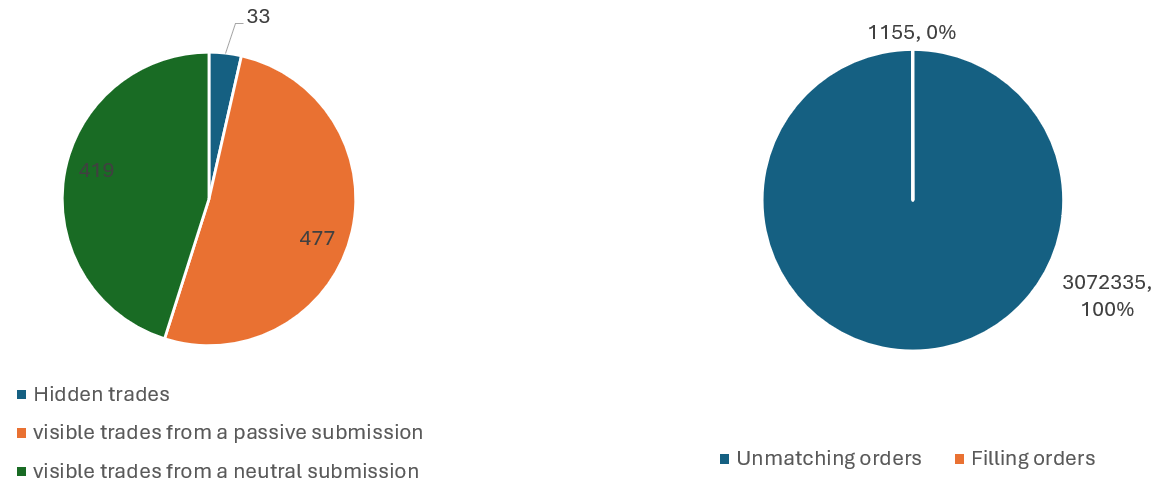
\includegraphics[width=0.8\linewidth]{figures/percentage_of_AT_unmatch.png}
    \caption{Percentage of Passive and Neutral Orders getting filled in the Trade Book and Orders Filled vs. Unmatched in the Order Book}
    \label{fig:p_of_AT_unma}
\end{figure}


\section{Prices and Filling Information} \label{sec:price}
To have a comprehensive understanding of how trades in trade book correspond to orders in order book, Figure~\ref{fig:p_f_i} provides an overview of the whole active trading hours from 10 am to 4 pm on 31st January. This date is chosen for demonstration, and the time window is the active trading time range during the day. This plot shows how filled price in the trade book track the mid-price in the order book, the distribution of passive and aggressive trades, and the spread range for each trade (not each order). The lower subplot presents the filled volume for each trading record.

% \begin{figure}[ht]
%     \centering
%     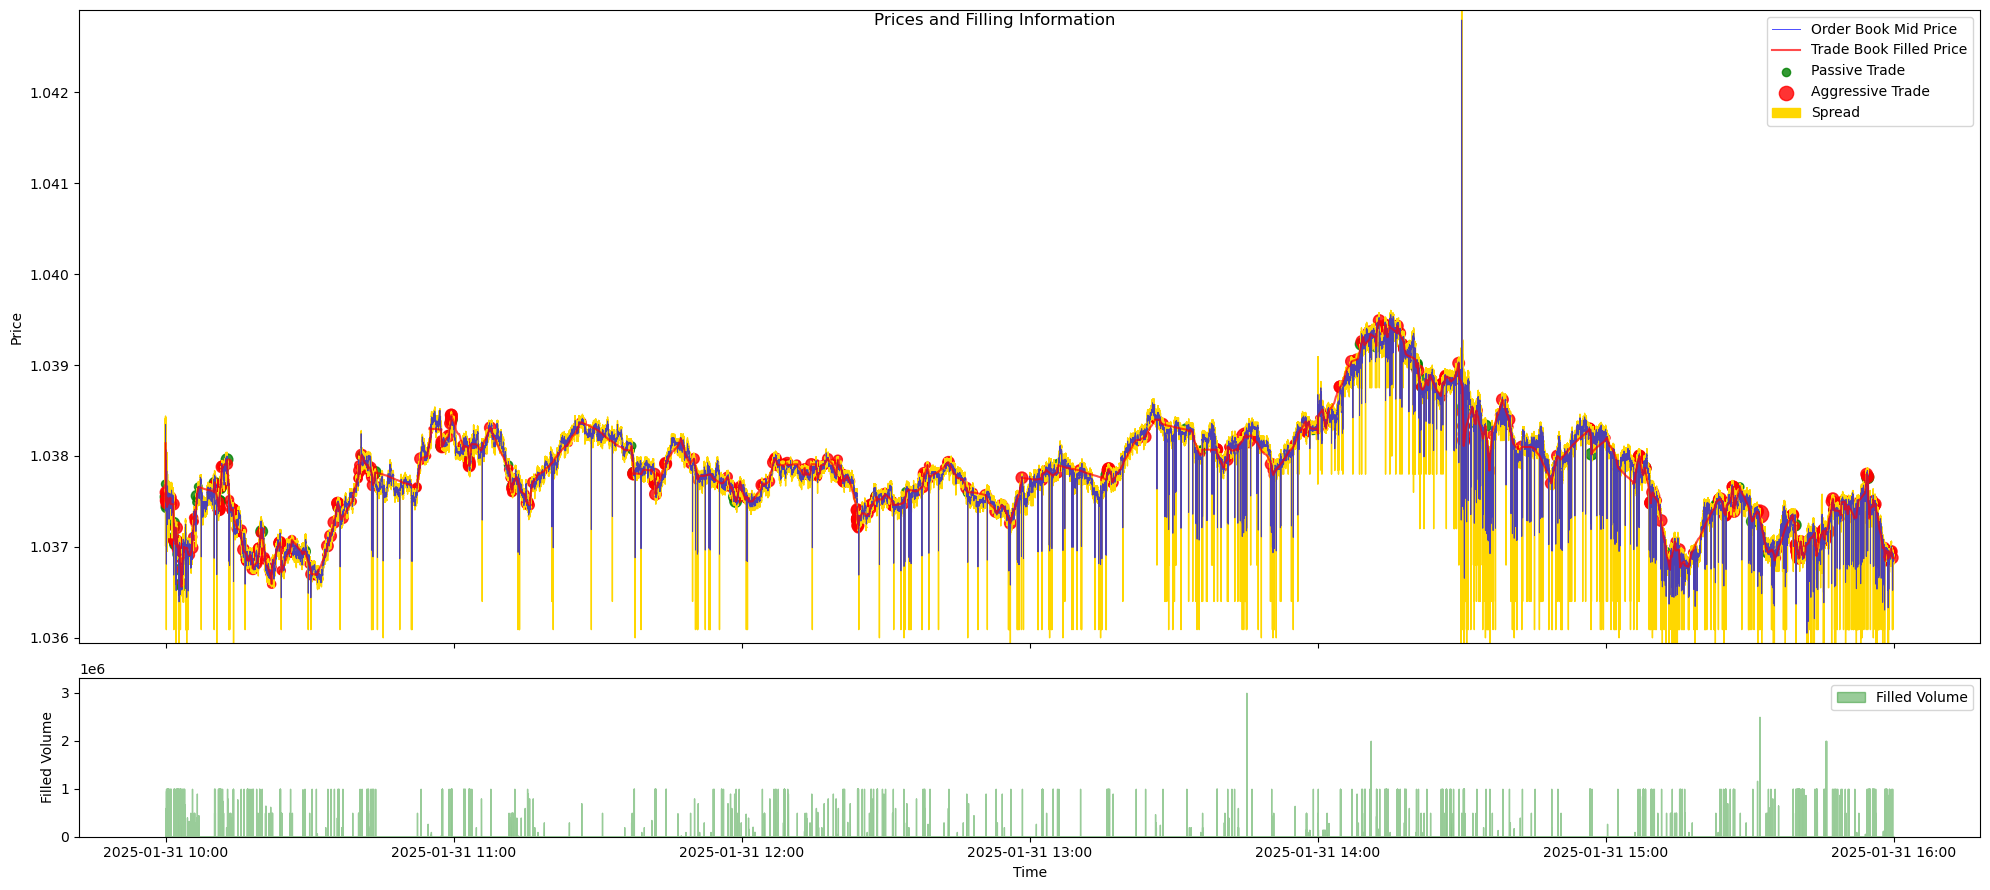
\includegraphics[width=1\linewidth]{figures/Prices and Filling Information.png}
%     \caption{Prices and filling information. This plot shows the mid-price from the order book (blue line), trade book filled prices (red line), and spread (yellow shading). Passive trades (green dots) and aggressive trades (red dots) are highlighted. The bottom panel represents the filled volume over time.}
%     \label{fig:p_f_i}
% \end{figure}


As can be seen in Figure~\ref{fig:p_f_i}, the mid-price has the highest point between 14:00 and 15:00. The filled price fits the mid-price well. We can see there are a lot of red dots which shows that they are aggressive trades. We did not classify bid or ask side because it's not the research target in the thesis. These aggressive trades go outside the spread range. The size of dots stands for relative volume of the trades. In other words, when the volume is large compared to other timestamps, the size of the dot will be larger. Therefore, we can easily see the active trading time point in the plot. Moreover, red dots represent aggressive trades in the trade book. We can see the red dots are more than green ones, which indicates that a lot of orders get filled by aggressive traders taking out them of the order book, instead of passively waiting for the market movements. This aligns with our need to improve the backtesting environment by predicting aggressive trades across the order book. Specially, there are several sparks in the trend of mid-price in the order book. Their frequent appearance in the plot suggests a systematic market behavior rather than random noise. These are caused by sudden jump in the best bid/ask price. As can be seen, most of them are downside sparks, which indicates that it seems the ask stays relatively stable while the bid collapses. This could be the reason that leads to sharp drops in mid-price.

From the bottom panel, in the beginning of 10:00, 15:45, 14:11, there are high volume up to 2,000,000, which are higher than common volume 1,000,000. At 13:45, the highest trading volume occurs as 3,000,000. Combined the two plots together, we can see when there's a drop, it's often accompanied by many trading records or large trades. 

In the Figure~\ref{fig:f_p_f_i} after filtering 2,381 sparks in the data, we can clearly see the price trends and some clustering for aggressive trades. For example, Table~\ref{tab:trade_sample} shows in the beginning of 10:00, many aggressive trades gather here. It may because there is a sharp dropping movement in the market, which triggers a wave of aggressive sell orders that consume the top levels of the bid side. This sudden removal of liquidity causes the mid-price to drop quickly, and encourages further aggressive selling or stop-loss execution.  

\begin{table}[htbp]
\centering
    \begin{tabular}{lcccccc}
    \toprule
    \textbf{Index} & \textbf{TIMESTAMP} & \textbf{$\bar{\alpha}$} & \textbf{FPRICE} & \textbf{FVOLUME} & \textbf{SPREAD} & \textbf{MID-PRICE} \\
    \midrule
    0  & 2025-01-31 10:00:00.007 & NaN & NaN   & 0.0      & 0.00042 & 1.037930 \\
    1  & 2025-01-31 10:00:00.012 & 1 & 1.038080 & 10000.0  & 0.00042 & 1.037930 \\
    2  & 2025-01-31 10:00:00.012 & 1 & 1.038140 & 1990000.0 & 0.00042 & 1.037930 \\
    3  & 2025-01-31 10:00:00.012 & 1 & 1.038140 & 10000.0  & 0.00042 & 1.037930 \\
    4  & 2025-01-31 10:00:00.017 & NaN & NaN & 0.0      & 0.00023 & 1.038325 \\
    5  & 2025-01-31 10:00:00.027 & NaN & NaN & 0.0      & 0.00007 & 1.038345 \\
    \vdots & \vdots & \vdots & \vdots & \vdots & \vdots & \vdots \\
    22 & 2025-01-31 10:00:00.195 & 1 & 1.037790 & 14841.0  & 0.00049 & 1.037745 \\
    23 & 2025-01-31 10:00:00.197 & NaN & NaN & 0.0      & 0.00054 & 1.037770 \\
    24 & 2025-01-31 10:00:00.205 & 1 & 1.037500 & 200000.0 & 0.00054 & 1.037770 \\
    25 & 2025-01-31 10:00:00.205 & 1 & 1.037500 & 180000.0 & 0.00054 & 1.037770 \\
    \vdots & \vdots & \vdots & \vdots & \vdots & \vdots & \vdots \\
    47 & 2025-01-31 10:00:00.417 & 0 & 1.037690 & 500000.0 & 0.00088 & 1.037980 \\
    % 48 & 2025-01-31 10:00:00.427 & NaN & 1.037680 & 0.0      & 0.00019 & 1.037635 \\
    % 49 & 2025-01-31 10:00:00.441 & NaN & 1.037670 & 0.0      & 0.00015 & 1.037615 \\
    \bottomrule
    \end{tabular}
\caption{Sample of Trades and Order Book Information. $\bar{\alpha}$ indicates the trade is aggressive (1), passive (0) or no-trade (NaN). FPRICE is filling price, FVOLUME is filling volume.}\label{tab:trade_sample}
\end{table}

\begin{sidewaysfigure}
    \centering
    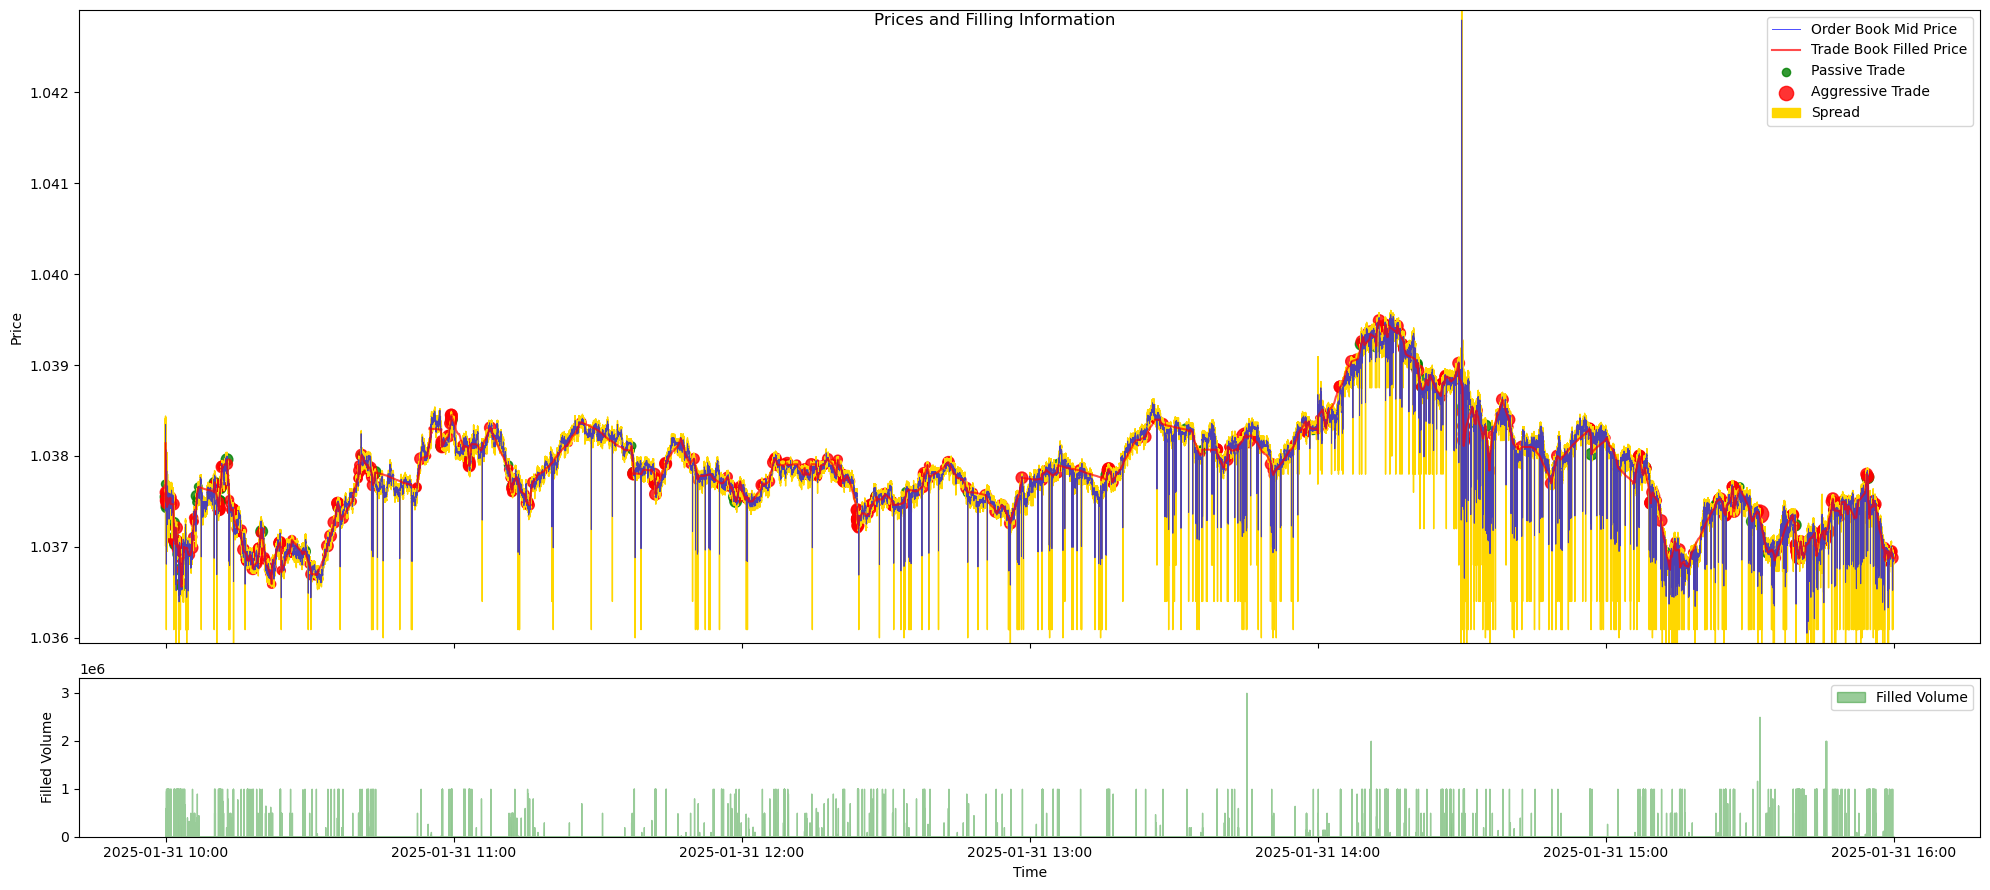
\includegraphics[width=\linewidth]{figures/Prices and Filling Information.png}
    \caption{Prices and filling information. This plot shows the mid-price from the order book (blue line), trade book filled prices (red line), and spread (yellow shading). Passive trades (green dots) and aggressive trades (red dots) are highlighted. The bottom panel represents the filled volume over time.}
    \label{fig:p_f_i}
\end{sidewaysfigure}

\begin{sidewaysfigure}
    \centering
    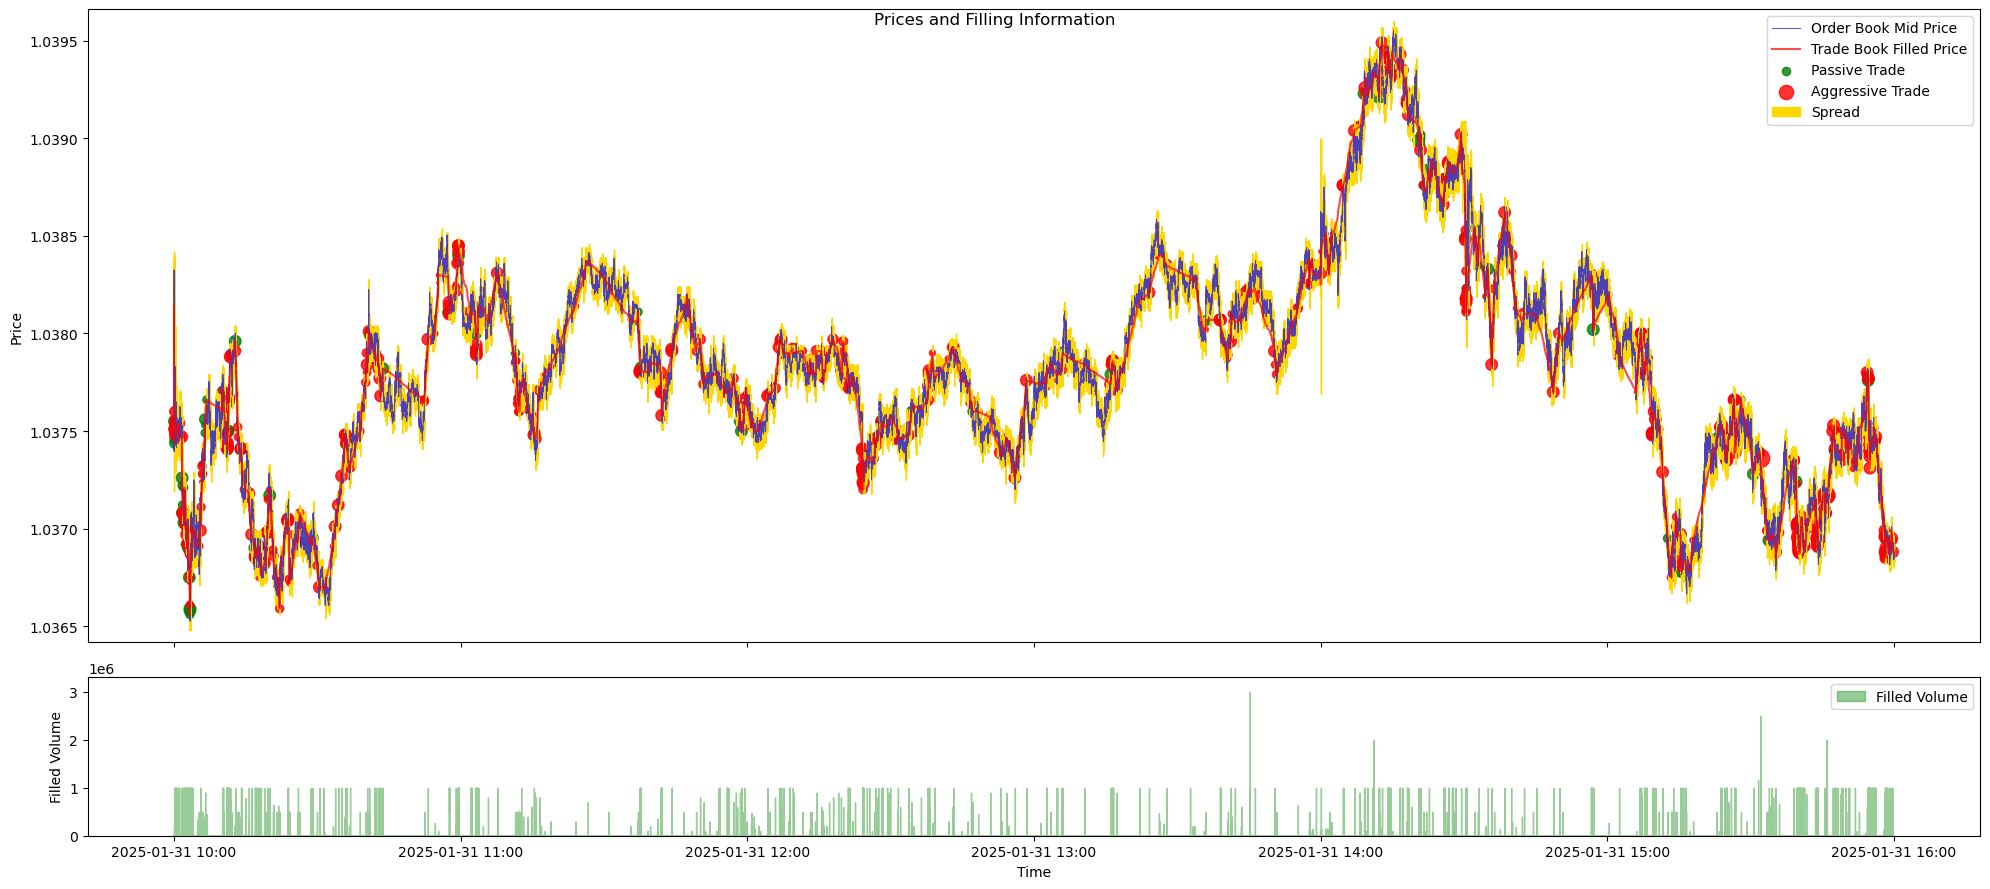
\includegraphics[width=\linewidth]{figures/Filtered Prices and Filling Information.png}
    \caption{Filtered prices and filling information. Similar to Figure~\ref{fig:p_f_i}, but filtering sharp jump points. This plot shows the mid-price from the order book (blue line), trade book filled prices (red line), and spread (yellow shading). Passive trades (green dots) and aggressive trades (red dots) are highlighted. The bottom panel represents the filled volume over time. The price and trade dynamics remain the same.}
    \label{fig:f_p_f_i}
\end{sidewaysfigure}



